%%%%%%%%%%%%%%%%%%%%%%%%%%%%%%%%%%%%%%%%%
% Stylish Article
% LaTeX Template
% Version 2.1 (1/10/15)
%
% This template has been downloaded from:
% http://www.LaTeXTemplates.com
%
% Original author:
% Mathias Legrand (legrand.mathias@gmail.com) 
% With extensive modifications by:
% Vel (vel@latextemplates.com)
%
% License:
% CC BY-NC-SA 3.0 (http://creativecommons.org/licenses/by-nc-sa/3.0/)
%
%%%%%%%%%%%%%%%%%%%%%%%%%%%%%%%%%%%%%%%%%

%----------------------------------------------------------------------------------------
%	PACKAGES AND OTHER DOCUMENT CONFIGURATIONS
%----------------------------------------------------------------------------------------

\documentclass[fleqn,10pt]{SelfArx} % Document font size and equations flushed left

\usepackage[english]{babel} % Specify a different language here - english by default

\usepackage{lipsum} % Required to insert dummy text. To be removed otherwise
\usepackage{hyperref}

%----------------------------------------------------------------------------------------
%	COLUMNS
%----------------------------------------------------------------------------------------

\setlength{\columnsep}{0.55cm} % Distance between the two columns of text
\setlength{\fboxrule}{0.75pt} % Width of the border around the abstract

%----------------------------------------------------------------------------------------
%	COLORS
%----------------------------------------------------------------------------------------

\definecolor{color1}{RGB}{0,0,90} % Color of the article title and sections
\definecolor{color2}{RGB}{0,20,20} % Color of the boxes behind the abstract and headings

%----------------------------------------------------------------------------------------
%	HYPERLINKS
%----------------------------------------------------------------------------------------

\usepackage{hyperref} % Required for hyperlinks
\hypersetup{hidelinks,colorlinks,breaklinks=true,urlcolor=color2,citecolor=color1,linkcolor=color1,bookmarksopen=false,pdftitle={Title},pdfauthor={Author}}

%----------------------------------------------------------------------------------------
%	ARTICLE INFORMATION
%----------------------------------------------------------------------------------------

\JournalInfo{CSCI-B565 Data Mining, Spring 2023} % Journal information
\Archive{} % Additional notes (e.g. copyright, DOI, review/research article)

\PaperTitle{Semester Project - Drug Discovery for Lung Cancer using Data Mining Techniques} % Article title

\Authors{\| Athulya Anand \| Diksha Adke \| Atharva Karnik \| Sricharraan Ramaswamy\textsuperscript{1}*} % Authors
\affiliation{\textsuperscript{1}\textit{Luddy School of Informatics, Computing, and Engineering, Indiana University, Bloomington, IN, USA}} % Author affiliation


\Keywords{\textit{Lung cancer, Small cell lung cancer, EGFR protein, Novel drugs, Efficacy prediction, Cancer cell proliferation, pIC50, Bioactivity class, Lipinski Descriptors, ML algorithms}} % Keywords - if you don't want any simply remove all the text between the curly brackets
\newcommand{\keywordname}{Keywords} % Defines the keywords heading name

%----------------------------------------------------------------------------------------
%	ABSTRACT
%----------------------------------------------------------------------------------------

\Abstract{Lung cancer remains a leading cause of cancer-related deaths worldwide, with small cell lung cancer (SCLC) being the most prevalent type. While conventional treatment modalities such as chemotherapy, radiation therapy, and surgery have demonstrated efficacy, their associated adverse effects have prompted the exploration of alternative lung cancer therapies, including novel drugs. Notably, the aberrant activation of the Epidermal Growth Factor Receptor (EGFR) protein is a crucial driver of lung cancer. In this project, we aim to evaluate the performance of various regression algorithms, namely Random Forest Regressor, Ada-boost Regressor, and Bagging Regressor, in predicting the efficacy of a drug in inhibiting the proliferation of cancer cells harboring EGFR protein defects.}

%----------------------------------------------------------------------------------------

\begin{document}

\flushbottom % Makes all text pages the same height

\maketitle % Print the title and abstract box

\tableofcontents % Print the contents section

\thispagestyle{empty} % Removes page numbering from the first page




%----------------------------------------------------------------------------------------
%Problem and Data Description
%----------------------------------------------------------------------------------------


\section{Problem and Data Description} % The \section*{} command stops section numbering
\subsection{Problem Statement}

 Lung cancer remains a leading cause of cancer-related deaths worldwide, with small cell lung cancer (SCLC) being the most prevalent type. Despite advances in the treatment of lung cancer, high mortality rates persist due to the limited efficacy and frequent negative side effects associated with current medications. Therefore, discovering novel therapeutics that are more effective, have fewer adverse effects, and can overcome drug resistance is crucial for improving treatment options for lung cancer patients. 

The abnormal activation of the Epidermal Growth Factor Receptor (EGFR) protein is a significant factor in the development and progression of lung cancer. The Epidermal Growth Factor Receptor (EGFR) is a protein responsible for facilitating cell growth and division. In cases of EGFR-positive lung cancer, a mutation or defect in the gene leads to continuous EGFR growth, causing uncontrolled cellular proliferation and ultimately, cancer. While chemotherapy remains one of the most effective solutions to treating cancer, its associated side effects such as fatigue, hair loss, and appetite changes have led to the exploration of alternative therapies. Specifically, various drugs are being tested for their efficacy in inhibiting EGFR protein multiplication. To measure a drug's efficiency in inhibiting EGFR protein growth, we utilized the Inhibitory Concentration (IC 50) value, a quantitative measure of the amount of drug required to inhibit a given biological process by 50 percent. In this project, we utilized the ChEMBL dataset, a chemical database of bioactive molecules, to obtain the canonical notation of molecular formulas for each drug. We then utilized the PubChem database to convert the canonical notation to molecular fingerprint, a unique binary representation of each molecule. We will implement machine learning models, namely Random Forest Regressor, Ada-boost Regressor, and Bagging Regressor, to predict the IC50 value for a given chemical. Our study aimed to compare the performance of these three models in predicting drug efficacy.

Thus, through this project we focus on solving the urgent need to enhance patient outcomes and lessen the burden of this illness serves as the driving force for a medication development endeavor for lung cancer. It provides the opportunity for substantial advancements in our understanding of lung cancer biology, improved treatment choices, higher survival rates, and better patient quality of life.
\subsection{Data Description}

The \textbf{\textit{ChEMBL dataset and Pubchem dataset}} has been utilized to obtain the necessary data for this study. It contains over 2 million curated bioactivity data entries, sourced from more than 76,000 documents and 1.2 million assays. The data covers 13,000 targets, 1,800 cells, and 33,000 indications. The version used for this study was ChEMBL version 26, as of March 25, 2020. 

The ChEMBL dataset is a curated chemical database that contains bioactive molecules with drug-like properties. It provides canonical notations of molecular formulas for each drug and integrates chemical, bioactivity, and genetic data to support the development of novel pharmaceuticals. 

In addition, the study utilizes the PubChem database, which includes data on small molecules as well as larger molecules such as nucleotides, carbohydrates, lipids, peptides, and chemically-modified macromolecules.

\bigskip

%----------------------------------------------------------------------------------------
%	Data Preprocessing $\&$ Exploratory Data Analysis
%----------------------------------------------------------------------------------------

\section{Data Preprocessing $\&$ Exploratory Data Analysis} % The \section*{} command stops section numbering


\subsection{Data Preprocessing: Handling Missing Values}
Data collection for this study began with a targeted search for 'EGFR' molecules within the ChEMBL database. The focus was on 'Single Protein' target types, and the molecular id corresponding to the human-specific type was extracted. The resulting dataset was then mined for samples with the standard type of 'IC50' to obtain a comprehensive understanding of the bioactivity data. 

To ensure the quality of the data, data pre-processing was conducted to remove missing values and duplicates, and compounds were classified and labeled according to their appropriate bioactivity thresholds. Following which, each compound was classified based on the bioactivity class namely \textbf{\textit{active, intermediate and inactive}}. The resulting data with the bioactivity curation is used for the further processes. 
\subsection{Exploratory Data Analysis}
Following the data preprocessing step in the earlier step, the next step involves conducting 'Exploratory Data Analysis' to gain insights into the data. The dataset consists of the molecular id, its corresponding canonical formula in the form of 'SMILE', and the 'IC 50' value indicating the bioactivity data. \textbf{\textit{Lipinski's rule}} of five is applied to the canonical formula to determine if the chemical compound is an active drug in humans. The rule states the following:
\begin{itemize}
    \item [a] The partition coefficient or 'log p' value should not exceed 5
    \item [b] There should be no more than 5 hydrogen bond donors
    \item [c] There should be no more than 10 hydrogen bond acceptors
    \item [c] The molecular mass should not exceed 500 daltons
\end{itemize}

To conform to the above-mentioned criteria, the logarithm of the ‘IC 50’ value is computed to the negative logarithmic scale which is essentially -log10(IC50) and recorded as ‘pIC50’. A function is then created to test the molecule with the given Lipinski descriptors using its canonical formula. The Lipinski descriptors in our case are ['MW', 'LogP', 'NumHDonors', 'NumHAcceptors']. Subsequently, exploratory data analysis is carried out on the dataset, utilizing ‘pIC50’ as the selection criteria and the Lipinksi descriptors. The results indicate that ‘pIC50’ is the primary measure used to distinguish active, intermediate and inactive compounds.

Fig 1., is a histogram plot showing the distribution of the pIC50 variable in the dataset with 20 bins. From the plot, we can infer the following:
\begin{figure}[h!]
    \centering
    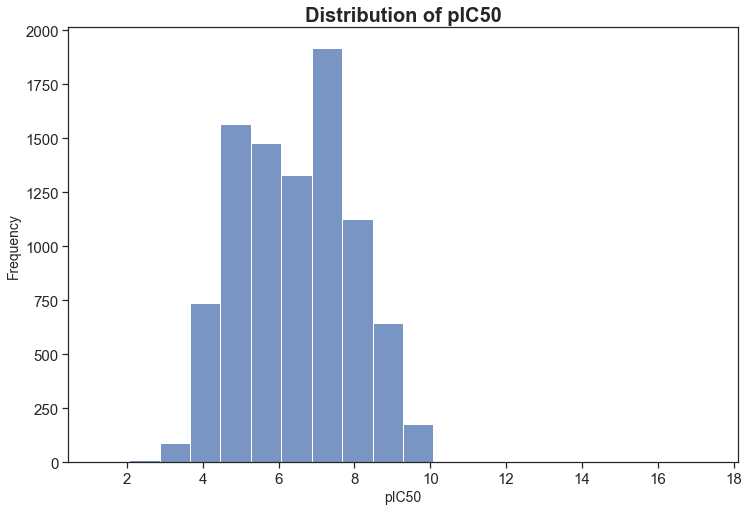
\includegraphics[width = 80mm, height = 50mm]{Milestone - I/1.png}
    \caption{Frequency distribution of pIC50}
    \label{fig:Frequency distribution of pIC50}
\end{figure}

The distribution of pIC50 appears to be slightly skewed to the right. The majority of the compounds have a pIC50 value between 5 and 8. There are very few compounds with pIC50 values less than 4. The distribution has a long tail to the right, indicating the presence of outliers with higher pIC50 values. 

\begin{figure}[h!]
    \centering
    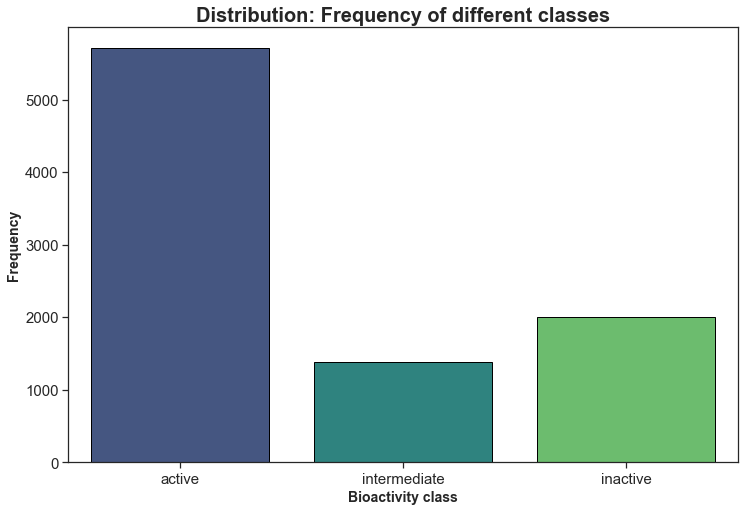
\includegraphics[width = 82mm, height = 53mm]{Milestone - I/2.png}
    \caption{Frequency distribution of Bioactivity classes}
    \label{fig:Frequency distribution of Bioactivity classes}
\end{figure}

From Fig2., countplot, The most common bioactivity class is "active," followed by "inactive" and "intermediate." The distribution of bioactivity classes is not evenly spread and so, we move on to perform EDA on the Lipinksi descriptors to find credible results. 
\subsubsection{Exploratory Data Analysis via Lipinski Descriptors}
\begin{figure}[h!]
    \centering
    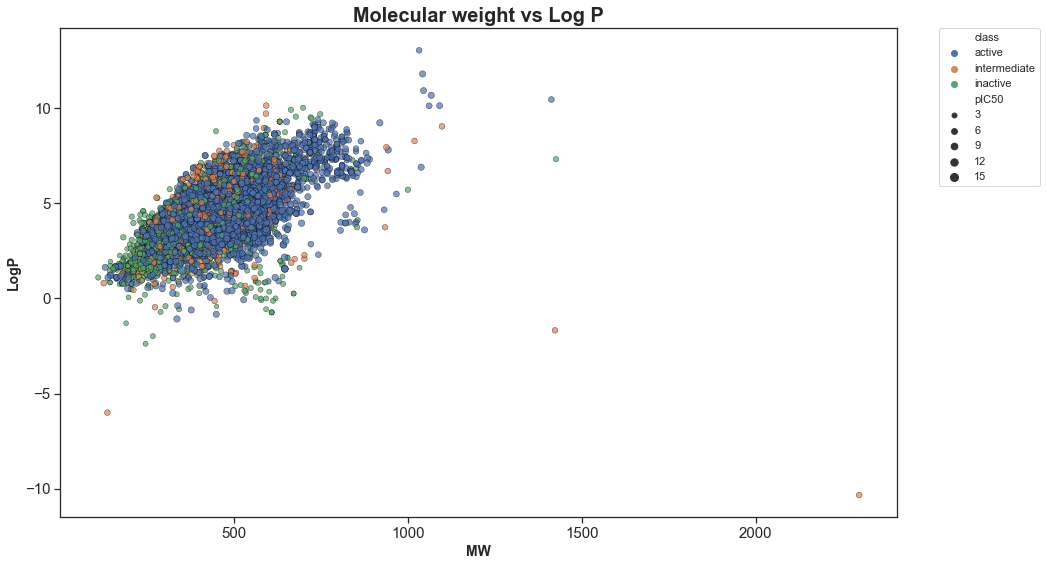
\includegraphics[width = 94mm, height = 53mm]{Milestone - I/3.png}
    \caption{Scatter Plot: Molecular Weight vs Log P}
    \label{fig:Scatter Plot: Molecular Weight vs Log P}
\end{figure}

Fig 3., suggests that the majority of compounds in the dataset have a MW below 1000 and a LogP value between -2 and 6. The size of the data points represents the pIC50 value, with larger points indicating compounds with higher potency. The color of the data points represents the bioactivity class, with inactive compounds represented by green, active compounds by blue, and intermediate compounds by orange. With the huge cluster of datapoints there seems to be no clear correlation between MW and LogP with respect to bioactivity class or potency, suggesting that other factors may be more important in determining bioactivity.



\begin{figure}[h!]
    \centering
    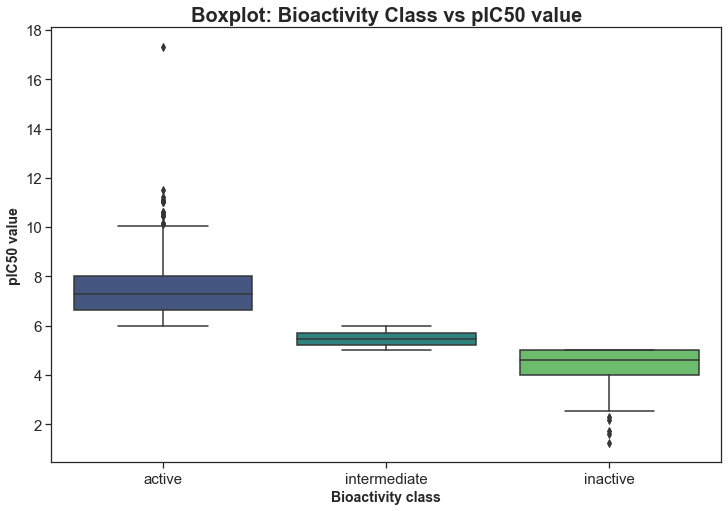
\includegraphics[width = 80mm, height = 53mm]{Milestone - I/4.png}
    \caption{Box Plot: Bioactivity Class vs pIC50}
    \label{fig:Box Plot: Bioactivity Class vs pIC50}
\end{figure}
Let us now have a comparitive study between the bioactivity classes and each Lipinski descriptor using EDA. 
\\\\\\\\\\\\
\begin{figure}[ht]
  \centering
  \subfigure{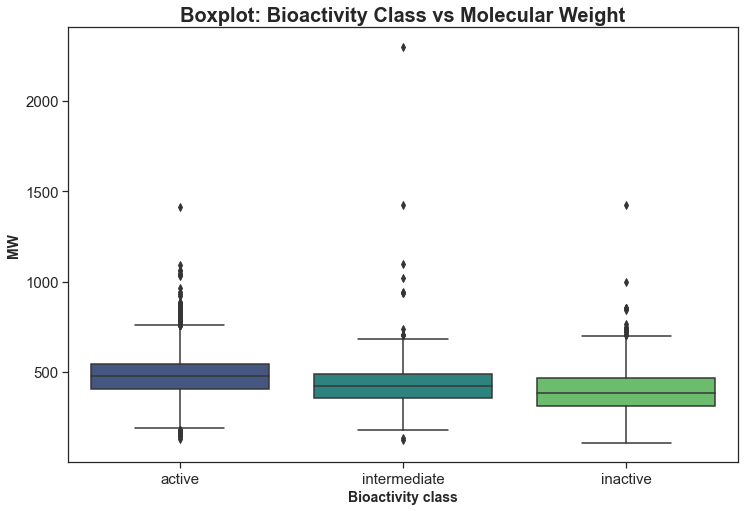
\includegraphics[width=0.5\linewidth]{Milestone - I/5.png}}\hfill
  \subfigure{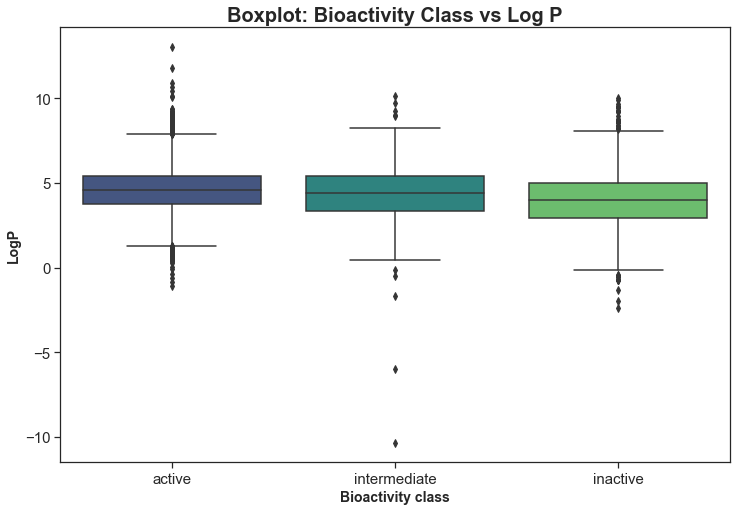
\includegraphics[width=0.5\linewidth]{Milestone - I/6.png}}\\
  \subfigure{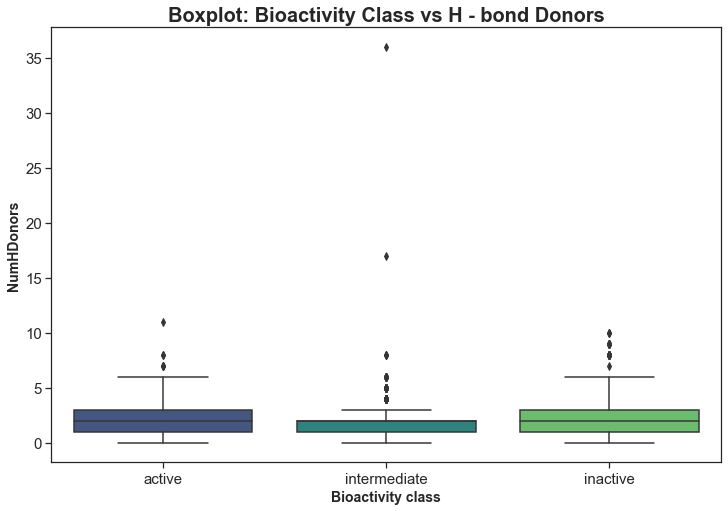
\includegraphics[width=0.5\linewidth]{Milestone - I/7.png}}\hfill
  \subfigure{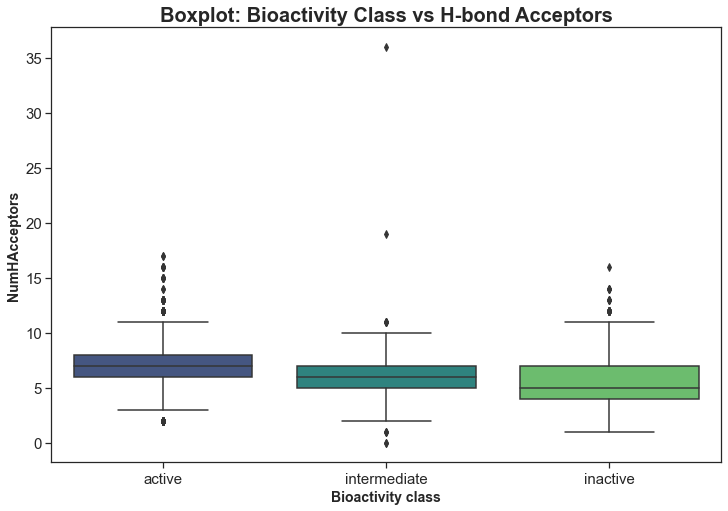
\includegraphics[width=0.5\linewidth]{Milestone - I/8.png}}
  \caption{Bioactivity Class with Lipinski Descriptors}
  \label{Bioactivity Class with Lipinski Descriptors}
\end{figure}

From the above subplot, we can analyze the bioactivity class for each lipinski descriptor and see that the median value for each is very variant. This can be slightly tedious and so we plot a pairplot between each and every descriptor along with the pIC50 values to see if any constructive analysis can be made. 

\begin{figure}[h!]
    \centering
    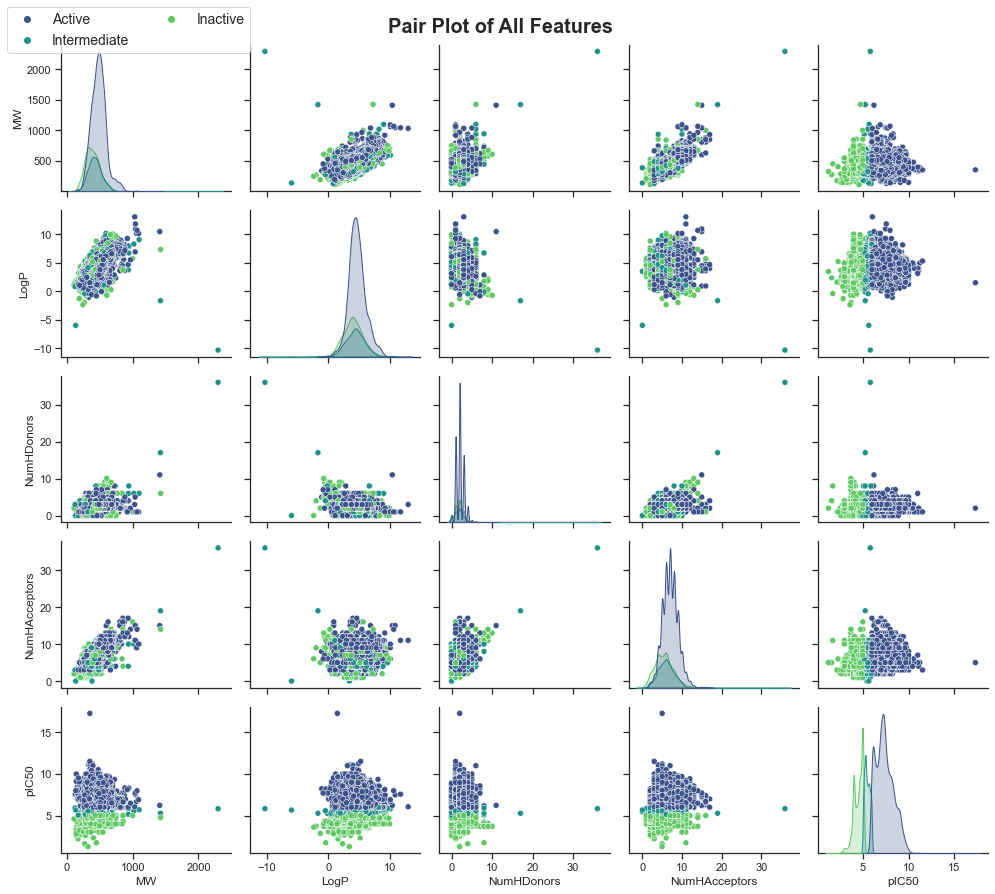
\includegraphics[width = 90mm, height = 87mm]{Milestone - I/9.png}
    \caption{Pair plot of all factors}
    \label{fig:Pair plot of all factors}
\end{figure}

Fig 9., suggests that the 2 bioactivity classes are spanning similar chemical spaces as evident by the scatter plot of MW vs LogP in Fig 3.
\\\\\\\\\\\\\\\\\
Lastly, we perform Pearsons Correlation between pIC50 and all the Lipinksi descriptor to check the mos highly correlated factors thereby concluding the best features to be selected in the future steps of the project. 
\begin{figure}[h!]
    \centering
    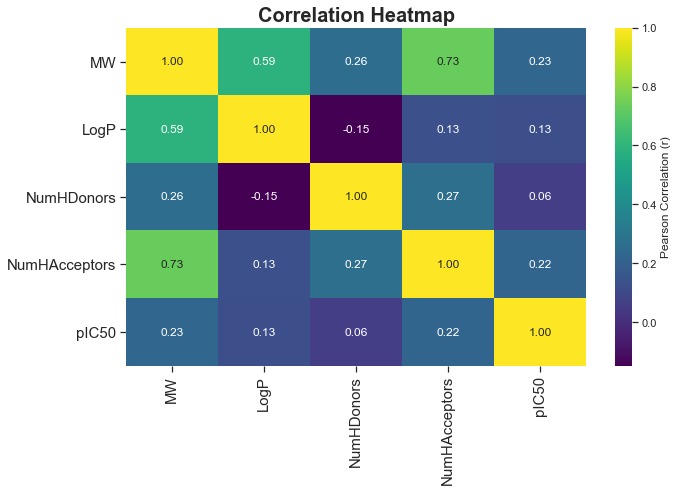
\includegraphics[width = 90mm, height = 70mm]{Milestone - I/10.png}
    \caption{Correlation heatmap of all features}
    \label{fig:Correlation heatmap of all features}
\end{figure}

Fig10., depicts that there is a low degree of correlation observed among the features in the dataset, with the exception of NumHAcceptors and molecular weight, which display a significant and strong positive correlation. Therefore, we have decided to retain all the features in the analysis.
\bigskip
\bigskip
%----------------------------------------------------------------------------------------
 % Algorithm and Methodology
%----------------------------------------------------------------------------------------

\section{Algorithm and Methodology}

Add subsections if needed.

\bigskip
\bigskip
%----------------------------------------------------------------------------------------
 % Experiments and Results
%----------------------------------------------------------------------------------------
\section{Experiments and Results}


\bigskip
\bigskip

%----------------------------------------------------------------------------------------
 %Deployement
%----------------------------------------------------------------------------------------
\section{Deployment and Maintenance}


\bigskip
\bigskip

%----------------------------------------------------------------------------------------
 % Summary and Conclusions
%----------------------------------------------------------------------------------------
\section{Summary and Conclusions}
\bigskip
\bigskip
\bigskip


\phantomsection
\section*{Acknowledgments} % The \section*{} command stops section numbering
We extend our appreciation to the authors of the datasets used in this project for making their data publicly available. Additionally, we also extend our gratitude to Dr. Hasan Kurban, AI's and TA's for their constant support and guidance through the execution of this project. 
\addcontentsline{toc}{section}{Acknowledgments} % Adds this section to the table of contents

%----------------------------------------------------------------------------------------
%	REFERENCE LIST
%----------------------------------------------------------------------------------------
\phantomsection
\bibliographystyle{unsrt}
\bibliography{sample}
\begin{enumerate}
  \item \href{https://www.ebi.ac.uk/chembl/}{https://www.ebi.ac.uk/chembl/}
  \item \href{https://pubchem.ncbi.nlm.nih.gov/docs/about}{https://pubchem.ncbi.nlm.nih.gov/docs/about}
  \item \href{https://www.ncbi.nlm.nih.gov/pmc/articles/PMC3245175/}{https://www.ncbi.nlm.nih.gov/pmc/articles/PMC3245175/}
  \item \href{https://en.wikipedia.org/wiki/Small-cell_carcinoma#Small-cell_lung_cancer}{https://en.wikipedia.org/wiki/Small-cell_carcinoma#Small-cell_lung_cancer}
\end{enumerate}
%----------------------------------------------------------------------------------------

\end{document}